\documentclass{beamer}
\usetheme{default}

\usetheme{default}
% Slide setup, colour independent

\usepackage{amsmath,amssymb,amsthm}
\usepackage{colortbl}
\usepackage{bm}
\usepackage{xcolor}
\usepackage{dsfont}
\usepackage{setspace}
%\usepackage{subfigure}
% To use \ding{234} and the like
\usepackage{pifont}
% To cross reference between slide files
\usepackage{zref-xr,zref-user}
% Use something like
% \zexternaldocument{fileI}
% in the tex files. And cite using \zref instead of \ref

% Fields and the like
\def\IC{\mathbb{C}}
\def\IF{\mathbb{F}}
\def\II{\mathbb{I}}
\def\IJ{\mathbb{J}}
\def\IM{\mathbb{M}}
\def\IN{\mathbb{N}}
\def\IP{\mathbb{P}}
\def\IR{\mathbb{R}}
\def\IZ{\mathbb{Z}}
\def\11{\mathds{1}}


% Bold lowercase
\def\ba{\mathbf{a}}
\def\bb{\mathbf{b}}
\def\bc{\mathbf{c}}
\def\bd{\mathbf{d}}
\def\be{\mathbf{e}}
\def\bf{\mathbf{f}}
\def\bh{\mathbf{h}}
\def\bi{\mathbf{i}}
\def\bj{\mathbf{j}}
\def\bk{\mathbf{k}}
\def\bn{\mathbf{n}}
\def\bp{\mathbf{p}}
\def\br{\mathbf{r}}
\def\bs{\mathbf{s}}
\def\bu{\mathbf{u}}
\def\bv{\mathbf{v}}
\def\bw{\mathbf{w}}
\def\bx{\mathbf{x}}
\def\by{\mathbf{y}}
\def\bz{\mathbf{z}}

% Bold capitals
\def\bB{\mathbf{B}}
\def\bD{\mathbf{D}}
\def\bF{\mathbf{F}}
\def\bG{\mathbf{G}}
\def\bI{\mathbf{I}}
\def\bL{\mathbf{L}}
\def\bN{\mathbf{N}}
\def\bP{\mathbf{P}}
\def\bR{\mathbf{R}}
\def\bS{\mathbf{S}}
\def\bT{\mathbf{T}}
\def\bX{\mathbf{X}}

% Bold numbers
\def\b0{\mathbf{0}}

% Bold greek
\bmdefine{\bmu}{\bm{\mu}}
\def\bphi{\bm{\phi}}
\def\bvarphi{\bm{\varphi}}

% Bold red sentence
\def\boldred#1{{\color{red}\textbf{#1}}}
\def\defword#1{{\color{orange}\textbf{#1}}}

% Caligraphic letters
\def\A{\mathcal{A}}
\def\B{\mathcal{B}}
\def\C{\mathcal{C}}
\def\D{\mathcal{D}}
\def\E{\mathcal{E}}
\def\F{\mathcal{F}}
\def\G{\mathcal{G}}
\def\H{\mathcal{H}}
\def\I{\mathcal{I}}
\def\L{\mathcal{L}}
\def\M{\mathcal{M}}
\def\N{\mathcal{N}}
\def\P{\mathcal{P}}
\def\R{\mathcal{R}}
\def\S{\mathcal{S}}
\def\T{\mathcal{T}}
\def\U{\mathcal{U}}
\def\V{\mathcal{V}}

% tt font for code
\def\code#1{{\tt #1}}

% i.e., e.g.
\def\eg{\emph{e.g.}}
\def\ie{\emph{i.e.}}


% Operators and special symbols
\def\nbOne{{\mathchoice {\rm 1\mskip-4mu l} {\rm 1\mskip-4mu l}
{\rm 1\mskip-4.5mu l} {\rm 1\mskip-5mu l}}}
\def\cov{\ensuremath{\mathsf{cov}}}
\def\Var{\ensuremath{\mathsf{Var}\ }}
\def\Im{\textrm{Im}\;}
\def\Re{\textrm{Re}\;}
\def\det{\ensuremath{\mathsf{det}}}
\def\diag{\ensuremath{\mathsf{diag}}}
\def\nullspace{\ensuremath{\mathsf{null}}}
\def\nullity{\ensuremath{\mathsf{nullity}}}
\def\rank{\ensuremath{\mathsf{rank}}}
\def\range{\ensuremath{\mathsf{range}}}
\def\sgn{\ensuremath{\mathsf{sgn}}}
\def\Span{\ensuremath{\mathsf{span}}}
\def\tr{\ensuremath{\mathsf{tr}}}
\def\imply{$\Rightarrow$}
\def\restrictTo#1#2{\left.#1\right|_{#2}}
\newcommand{\parallelsum}{\mathbin{\!/\mkern-5mu/\!}}
\def\dsum{\mathop{\displaystyle \sum }}%
\def\dind#1#2{_{\substack{#1\\ #2}}}

\DeclareMathOperator{\GL}{GL}
\DeclareMathOperator{\Rel}{Re}
\def\Nt#1{\left|\!\left|\!\left|#1\right|\!\right|\!\right|}
\newcommand{\tripbar}{|\! |\! |}



% The beamer bullet (in base colour)
\def\bbullet{\leavevmode\usebeamertemplate{itemize item}\ }

% Theorems and the like
\newtheorem{proposition}[theorem]{Proposition}
\newtheorem{property}[theorem]{Property}
\newtheorem{importantproperty}[theorem]{Property}
\newtheorem{importanttheorem}[theorem]{Theorem}
%\newtheorem{lemma}[theorem]{Lemma}
%\newtheorem{corollary}[theorem]{Corollary}
\newtheorem{remark}[theorem]{Remark}
\setbeamertemplate{theorems}[numbered]
%\setbeamertemplate{theorems}[ams style]

%
%\usecolortheme{orchid}
%\usecolortheme{orchid}

\def\red{\color[rgb]{1,0,0}}
\def\blue{\color[rgb]{0,0,1}}
\def\green{\color[rgb]{0,1,0}}


% Get rid of navigation stuff
\setbeamertemplate{navigation symbols}{}

% Set footline/header line
\setbeamertemplate{footline}
{%
\quad p. \insertpagenumber \quad--\quad \insertsection\vskip2pt
}
% \setbeamertemplate{headline}
% {%
% \quad\insertsection\hfill p. \insertpagenumber\quad\mbox{}\vskip2pt
% }


\makeatletter
\newlength\beamerleftmargin
\setlength\beamerleftmargin{\Gm@lmargin}
\makeatother

% Colours for special pages
\def\extraContent{yellow!20}


%%%%%%%%%%%%%%%%%
\usepackage{tikz}
\usetikzlibrary{shapes,arrows}
\usetikzlibrary{positioning}
\usetikzlibrary{shapes.symbols,shapes.callouts,patterns}
\usetikzlibrary{calc,fit}
\usetikzlibrary{backgrounds}
\usetikzlibrary{decorations.pathmorphing,fit,petri}
\usetikzlibrary{automata}
\usetikzlibrary{fadings}
\usetikzlibrary{patterns,hobby}

\usetikzlibrary{backgrounds,fit,petri}


\usepackage{pgfplots}
\pgfplotsset{compat=1.6}
\pgfplotsset{ticks=none}

\usetikzlibrary{decorations.markings}
\usetikzlibrary{arrows.meta}
\tikzset{>=stealth}

% For tikz
\usetikzlibrary{shapes,arrows}
\usetikzlibrary{positioning}
\tikzstyle{cloud} = [draw, ellipse,fill=red!20, node distance=0.87cm,
minimum height=2em]
\tikzstyle{line} = [draw, -latex']


%%% For max frame images
\newenvironment{changemargin}[2]{%
\begin{list}{}{%
\setlength{\topsep}{0pt}%
\setlength{\leftmargin}{#1}%
\setlength{\rightmargin}{#2}%
\setlength{\listparindent}{\parindent}%
\setlength{\itemindent}{\parindent}%
\setlength{\parsep}{\parskip}%
}%
\item[]}{\end{list}}


% Make one image take up the entire slide content area in beamer,.:
% centered/centred full-screen image, with title:
% This uses the whole screen except for the 1cm border around it
% all. 128x96mm
\newcommand{\titledFrameImage}[2]{
\begin{frame}{#1}
%\begin{changemargin}{-1cm}{-1cm}
\begin{center}
\includegraphics[width=108mm,height=\textheight,keepaspectratio]{#2}
\end{center}
%\end{changemargin}
\end{frame}
}

% Make one image take up the entire slide content area in beamer.:
% centered/centred full-screen image, no title:
% This uses the whole screen except for the 1cm border around it
% all. 128x96mm
\newcommand{\plainFrameImage}[1]{
\begin{frame}[plain]
%\begin{changemargin}{-1cm}{-1cm}
\begin{center}
\includegraphics[width=108mm,height=76mm,keepaspectratio]{#1}
\end{center}
%\end{changemargin}
\end{frame}
}

% Make one image take up the entire slide area, including borders, in beamer.:
% centered/centred full-screen image, no title:
% This uses the entire whole screen
\newcommand{\maxFrameImage}[1]{
\begin{frame}[plain]
\begin{changemargin}{-1cm}{-1cm}
\begin{center}
\includegraphics[width=\paperwidth,height=\paperheight,keepaspectratio]
{#1}
\end{center}
\end{changemargin}
\end{frame}
}

% This uses the entire whole screen (to include in frame)
\newcommand{\maxFrameImageNoFrame}[1]{
\begin{changemargin}{-1cm}{-1cm}
\begin{center}
\includegraphics[width=\paperwidth,height=0.99\paperheight,keepaspectratio]
{#1}
\end{center}
\end{changemargin}
}

% Make one image take up the entire slide area, including borders, in beamer.:
% centered/centred full-screen image, no title:
% This uses the entire whole screen
\newcommand{\maxFrameImageColor}[2]{
\begin{frame}[plain]
\setbeamercolor{normal text}{bg=#2!20}
\begin{changemargin}{-1cm}{-1cm}
\begin{center}
\includegraphics[width=\paperwidth,height=\paperheight,keepaspectratio]
{#1}
\end{center}
\end{changemargin}
\end{frame}
}


\usepackage{tikz}
\usetikzlibrary{patterns,hobby}
\usepackage{pgfplots}
\pgfplotsset{compat=1.6}
\pgfplotsset{ticks=none}

\usetikzlibrary{backgrounds}
\usetikzlibrary{decorations.markings}
\usetikzlibrary{arrows.meta}
\tikzset{>=stealth}

\tikzset{
  clockwise arrows/.style={
    postaction={
      decorate,
      decoration={
        markings,
        mark=between positions 0.1 and 0.9 step 40pt with {\arrow{>}},
   }}}}


   %%%%%%%%%%%
% To have links to parts in the outline
\makeatletter
\AtBeginPart{%
  \addtocontents{toc}{\protect\beamer@partintoc{\the\c@part}{\beamer@partnameshort}{\the\c@page}}%
}
%% number, shortname, page.
\providecommand\beamer@partintoc[3]{%
  \ifnum\c@tocdepth=-1\relax
    % requesting onlyparts.
    \makebox[6em]{Part #1:} \textcolor{green!30!blue}{\hyperlink{#2}{#2}}
    \par
  \fi
}
\define@key{beamertoc}{onlyparts}[]{%
  \c@tocdepth=-1\relax
}
\makeatother%

\newcommand{\nameofthepart}{}
\newcommand{\nupart}[1]%
    {   \part{#1}%
        \renewcommand{\nameofthepart}{#1}%
        {
          \setbeamercolor{background canvas}{bg=orange!50}
          \begin{frame}{#1}%\partpage 
          \hypertarget{\nameofthepart}{}\tableofcontents%
          \end{frame}
        }
    }



\usecolortheme{orchid}

%% Listings
\usepackage{listings}
\definecolor{mygreen}{rgb}{0,0.6,0}
\definecolor{mygray}{rgb}{0.5,0.5,0.5}
\definecolor{mymauve}{rgb}{0.58,0,0.82}
\definecolor{mygold}{rgb}{1,0.843,0}
\definecolor{myblue}{rgb}{0.537,0.812,0.941}

\definecolor{lgreen}{rgb}{0.6,0.9,.6}
\definecolor{lred}{rgb}{1,0.5,.5}

\lstloadlanguages{R}
\lstset{ %
  language=R,
  backgroundcolor=\color{black!05},   % choose the background color
  basicstyle=\footnotesize\ttfamily,        % size of fonts used for the code
  breaklines=true,                 % automatic line breaking only at whitespace
  captionpos=b,                    % sets the caption-position to bottom
  commentstyle=\color{mygreen},    % comment style
  escapeinside={\%*}{*)},          % if you want to add LaTeX within your code
  keywordstyle=\color{red},       % keyword style
  stringstyle=\color{mygold},     % string literal style
  keepspaces=true,
  columns=fullflexible,
  tabsize=4,
}
% Could also do (in lstset)
% basicstyle==\fontfamily{pcr}\footnotesize
\lstdefinelanguage{Renhanced}%
  {keywords={abbreviate,abline,abs,acos,acosh,action,add1,add,%
      aggregate,alias,Alias,alist,all,anova,any,aov,aperm,append,apply,%
      approx,approxfun,apropos,Arg,args,array,arrows,as,asin,asinh,%
      atan,atan2,atanh,attach,attr,attributes,autoload,autoloader,ave,%
      axis,backsolve,barplot,basename,besselI,besselJ,besselK,besselY,%
      beta,binomial,body,box,boxplot,break,browser,bug,builtins,bxp,by,%
      c,C,call,Call,case,cat,category,cbind,ceiling,character,char,%
      charmatch,check,chol,chol2inv,choose,chull,class,close,cm,codes,%
      coef,coefficients,co,col,colnames,colors,colours,commandArgs,%
      comment,complete,complex,conflicts,Conj,contents,contour,%
      contrasts,contr,control,helmert,contrib,convolve,cooks,coords,%
      distance,coplot,cor,cos,cosh,count,fields,cov,covratio,wt,CRAN,%
      create,crossprod,cummax,cummin,cumprod,cumsum,curve,cut,cycle,D,%
      data,dataentry,date,dbeta,dbinom,dcauchy,dchisq,de,debug,%
      debugger,Defunct,default,delay,delete,deltat,demo,de,density,%
      deparse,dependencies,Deprecated,deriv,description,detach,%
      dev2bitmap,dev,cur,deviance,off,prev,,dexp,df,dfbetas,dffits,%
      dgamma,dgeom,dget,dhyper,diag,diff,digamma,dim,dimnames,dir,%
      dirname,dlnorm,dlogis,dnbinom,dnchisq,dnorm,do,dotplot,double,%
      download,dpois,dput,drop,drop1,dsignrank,dt,dummy,dump,dunif,%
      duplicated,dweibull,dwilcox,dyn,edit,eff,effects,eigen,else,%
      emacs,end,environment,env,erase,eval,equal,evalq,example,exists,%
      exit,exp,expand,expression,External,extract,extractAIC,factor,%
      fail,family,fft,file,filled,find,fitted,fivenum,fix,floor,for,%
      For,formals,format,formatC,formula,Fortran,forwardsolve,frame,%
      frequency,ftable,ftable2table,function,gamma,Gamma,gammaCody,%
      gaussian,gc,gcinfo,gctorture,get,getenv,geterrmessage,getOption,%
      getwd,gl,glm,globalenv,gnome,GNOME,graphics,gray,grep,grey,grid,%
      gsub,hasTsp,hat,heat,help,hist,home,hsv,httpclient,I,identify,if,%
      ifelse,Im,image,\%in\%,index,influence,measures,inherits,install,%
      installed,integer,interaction,interactive,Internal,intersect,%
      inverse,invisible,IQR,is,jitter,kappa,kronecker,labels,lapply,%
      layout,lbeta,lchoose,lcm,legend,length,levels,lgamma,library,%
      licence,license,lines,list,lm,load,local,locator,log,log10,log1p,%
      log2,logical,loglin,lower,lowess,ls,lsfit,lsf,ls,machine,Machine,%
      mad,mahalanobis,make,link,margin,match,Math,matlines,mat,matplot,%
      matpoints,matrix,max,mean,median,memory,menu,merge,methods,min,%
      missing,Mod,mode,model,response,mosaicplot,mtext,mvfft,na,nan,%
      names,omit,nargs,nchar,ncol,NCOL,new,next,NextMethod,nextn,%
      nlevels,nlm,noquote,NotYetImplemented,NotYetUsed,nrow,NROW,null,%
      numeric,\%o\%,objects,offset,old,on,Ops,optim,optimise,optimize,%
      options,or,order,ordered,outer,package,packages,page,pairlist,%
      pairs,palette,panel,par,parent,parse,paste,path,pbeta,pbinom,%
      pcauchy,pchisq,pentagamma,persp,pexp,pf,pgamma,pgeom,phyper,pico,%
      pictex,piechart,Platform,plnorm,plogis,plot,pmatch,pmax,pmin,%
      pnbinom,pnchisq,pnorm,points,poisson,poly,polygon,polyroot,pos,%
      postscript,power,ppoints,ppois,predict,preplot,pretty,Primitive,%
      print,prmatrix,proc,prod,profile,proj,prompt,prop,provide,%
      psignrank,ps,pt,ptukey,punif,pweibull,pwilcox,q,qbeta,qbinom,%
      qcauchy,qchisq,qexp,qf,qgamma,qgeom,qhyper,qlnorm,qlogis,qnbinom,%
      qnchisq,qnorm,qpois,qqline,qqnorm,qqplot,qr,Q,qty,qy,qsignrank,%
      qt,qtukey,quantile,quasi,quit,qunif,quote,qweibull,qwilcox,%
      rainbow,range,rank,rbeta,rbind,rbinom,rcauchy,rchisq,Re,read,csv,%
      csv2,fwf,readline,socket,real,Recall,rect,reformulate,regexpr,%
      relevel,remove,rep,repeat,replace,replications,report,require,%
      resid,residuals,restart,return,rev,rexp,rf,rgamma,rgb,rgeom,R,%
      rhyper,rle,rlnorm,rlogis,rm,rnbinom,RNGkind,rnorm,round,row,%
      rownames,rowsum,rpois,rsignrank,rstandard,rstudent,rt,rug,runif,%
      rweibull,rwilcox,sample,sapply,save,scale,scan,scan,screen,sd,se,%
      search,searchpaths,segments,seq,sequence,setdiff,setequal,set,%
      setwd,show,sign,signif,sin,single,sinh,sink,solve,sort,source,%
      spline,splinefun,split,sqrt,stars,start,stat,stem,step,stop,%
      storage,strstrheight,stripplot,strsplit,structure,strwidth,sub,%
      subset,substitute,substr,substring,sum,summary,sunflowerplot,svd,%
      sweep,switch,symbol,symbols,symnum,sys,status,system,t,table,%
      tabulate,tan,tanh,tapply,tempfile,terms,terrain,tetragamma,text,%
      time,title,topo,trace,traceback,transform,tri,trigamma,trunc,try,%
      ts,tsp,typeof,unclass,undebug,undoc,union,unique,uniroot,unix,%
      unlink,unlist,unname,untrace,update,upper,url,UseMethod,var,%
      variable,vector,Version,vi,warning,warnings,weighted,weights,%
      which,while,window,write,\%x\%,x11,X11,xedit,xemacs,xinch,xor,%
      xpdrows,xy,xyinch,yinch,zapsmall,zip},%
   otherkeywords={!,!=,~,$,*,\%,\&,\%/\%,\%*\%,\%\%,<-,<<-,_,/},%
   alsoother={._$},%
   sensitive,%
   morecomment=[l]\#,%
   morestring=[d]",%
   morestring=[d]'% 2001 Robert Denham
  }%

%%%%%%% 
%% Definitions in yellow boxes
\usepackage{etoolbox}
\setbeamercolor{block title}{use=structure,fg=structure.fg,bg=structure.fg!40!bg}
\setbeamercolor{block body}{parent=normal text,use=block title,bg=block title.bg!20!bg}

\BeforeBeginEnvironment{definition}{%
	\setbeamercolor{block title}{fg=black,bg=yellow!20!white}
	\setbeamercolor{block body}{fg=black, bg=yellow!05!white}
}
\AfterEndEnvironment{definition}{
	\setbeamercolor{block title}{use=structure,fg=structure.fg,bg=structure.fg!20!bg}
	\setbeamercolor{block body}{parent=normal text,use=block title,bg=block title.bg!50!bg, fg=black}
}
\BeforeBeginEnvironment{importanttheorem}{%
	\setbeamercolor{block title}{fg=black,bg=red!20!white}
	\setbeamercolor{block body}{fg=black, bg=red!05!white}
}
\AfterEndEnvironment{importanttheorem}{
	\setbeamercolor{block title}{use=structure,fg=structure.fg,bg=structure.fg!20!bg}
	\setbeamercolor{block body}{parent=normal text,use=block title,bg=block title.bg!50!bg, fg=black}
}
\BeforeBeginEnvironment{importantproperty}{%
	\setbeamercolor{block title}{fg=black,bg=red!50!white}
	\setbeamercolor{block body}{fg=black, bg=red!30!white}
}
\AfterEndEnvironment{importantproperty}{
	\setbeamercolor{block title}{use=structure,fg=structure.fg,bg=structure.fg!20!bg}
	\setbeamercolor{block body}{parent=normal text,use=block title,bg=block title.bg!50!bg, fg=black}
}


% Beginning of a section
\AtBeginSection[]{
	{
		\setbeamercolor{background canvas}{bg=yellow!10}
		\begin{frame}[noframenumbering,plain]
			\framesubtitle{\nameofthepart Chapter \insertromanpartnumber \ -- \iteminsert{\insertpart}}
			\tableofcontents[
				currentsection,
				sectionstyle=show/shaded,
				subsectionstyle=show/show/hide]
		\end{frame}
	\addtocounter{page}{-1}
	%\addtocounter{framenumber}{-1} 
	}
}

% Beginning of a section
\AtBeginSubsection[]{
	{
		\setbeamercolor{background canvas}{bg=green!10}
		\begin{frame}[noframenumbering,plain]
				\framesubtitle{\nameofthepart Chapter \insertromanpartnumber \ -- \iteminsert{\insertpart}}
				\tableofcontents[
					currentsection,
					sectionstyle=show/hide,
					currentsubsection,
					subsectionstyle=show/shaded/hide]
			\end{frame}
		\addtocounter{page}{-1}
	}
}



\title{Matrix methods}
\date{}

\begin{document}
\DeclareFontShape{OT1}{cmss}{b}{n}{<->ssub * cmss/bx/n}{} 
\begin{frame}
	\titlepage
\end{frame}


%%%%%%%%%%%%%%%%%%%%%
%%%%%%%%%%%%%%%%%%%%%
%%%%%%%%%%%%%%%%%%%%%
%%%%%%%%%%%%%%%%%%%%%
\section{Orthogonality and projections}

\begin{frame}
\begin{definition}[Orthogonal set of vectors]
The set of vectors $\{\bv_1,\ldots,\bv_k\}\in\IR^n$ is an \textbf{orthogonal set} if
\[
\forall i,j=1,\ldots,k,\quad i\neq j \implies \bv_i\bullet\bv_j=0
\]
\end{definition}

\begin{theorem}\label{th:ortho_implies_LI}
$\{\bv_1,\ldots,\bv_k\}\in\IR^n$ with $\forall i$, $\bv_i\neq\b0$, orthogonal set $\implies$ $\{\bv_1,\ldots,\bv_k\}\in\IR^n$ linearly independent
\end{theorem}

\begin{definition}[Orthogonal basis]
Let $S$ be a basis of the subspace $W\subset\IR^n$ composed of an orthogonal set of vectors. We say $S$ is an \textbf{orthogonal basis} of $W$
\end{definition}
\end{frame}

\begin{frame}{Proof of Theorem~\ref{th:ortho_implies_LI}}
Assume $\{\bv_1,\ldots,\bv_k\}$ orthogonal set with $\bv_i\neq\b0$ for all $i=1,\ldots,k$. Recall $\{\bv_1,\ldots,\bv_k\}$ is LI if 
\[
c_1\bv_1+\cdots+c_k\bv_k=\b0\iff c_1=\cdots=c_k=0
\]
So assume $c_1,\ldots,c_k\in\IR$ are s.t. $c_1\bv_1+\cdots+c_k\bv_k=\b0$.
Recall that $\forall\bx\in\IR^k$, $\b0_k\bullet\bx=0$. So for some $\bv_i\in\{\bv_1,\ldots,\bv_k\}$
\begin{align}
0 &= \b0\bullet\bv_i \nonumber \\
&= (c_1\bv_1+\cdots+c_k\bv_k)\bullet\bv_i \nonumber \\
&= c_1\bv_1\bullet\bv_i+\cdots+c_k\bv_k\bullet\bv_i \label{eq:proof_th_ortho_implies_LI}
\end{align}
As $\{\bv_1,\ldots,\bv_k\}$ orthogonal, $\bv_j\bullet\bv_i=0$ when $i\neq j$, \eqref{eq:proof_th_ortho_implies_LI} reduces to
\[
c_i\bv_i\bullet\bv_i = 0 \iff c_i\|\bv_i\|^2 = 0
\]
As $\bv_i\neq 0$ for all $i$, $\|\bv_i\|\neq 0$ and so $c_i=0$. This is true for all $i$, hence the result
\end{frame}

\begin{frame}{Example -- Vectors of the standard basis of $\IR^3$}
For $\IR^3$, we denote
\[
\bi =\begin{pmatrix}
1\\0\\0
\end{pmatrix},\quad
\bj =\begin{pmatrix}
0\\1\\0
\end{pmatrix}
\textrm{ and }
\bk =\begin{pmatrix}
0\\0\\1
\end{pmatrix}
\]
($\IR^k$ for $k>3$, we denote them $\be_i$)
\vfill
Clearly, $\{\bi,\bj\}$, $\{\bi,\bk\}$, $\{\bj,\bk\}$ and $\{\bi,\bj,\bk\}$ orthogonal sets. The standard basis vectors are also $\neq\b0$, so the sets are LI. And
\[
\{\bi,\bj,\bk\}
\]
is an orthogonal basis of $\IR^3$ since it spans $\IR^3$ and is LI
\vfill
\[
c_1\bi+c_2\bj+c_3\bk
=
c_1\begin{pmatrix}
1\\0\\0
\end{pmatrix}
+c_2\begin{pmatrix}
0\\1\\0
\end{pmatrix}
+c_3\begin{pmatrix}
0\\0\\1
\end{pmatrix}
=
\begin{pmatrix}
c_1\\c_2\\c_3
\end{pmatrix}
\]
\end{frame}

\begin{frame}{Orthonormal version of things}
\begin{definition}[Orthonormal set]
The set of vectors $\{\bv_1,\ldots,\bv_k\}\in\IR^n$ is an \textbf{orthonormal set} if it is an orthogonal set and furthermore
\[
\forall i=1,\ldots,k,\quad \|\bv_i\|=1
\]
\end{definition}
\begin{definition}[Orthonormal basis]
A basis of the subspace $W\subset\IR^n$ is an \textbf{orthonormal basis} if the vectors composing it are an orthonormal set
\end{definition}
\vfill
$\{\bv_1,\ldots,\bv_k\}\in\IR^n$ is orthonormal if
\[
\bv_i\bullet\bv_j =
\begin{cases}
1 &\textrm{if }i=j \\
0 &\textrm{otherwise}
\end{cases}
\]
\end{frame}


\begin{frame}{Projections}
	\begin{definition}[Orthogonal projection onto a subspace]
	$W\subset\IR^n$ a subspace and $\{\bu_1,\ldots,\bu_k\}$ an orthogonal basis of $W$. $\forall\bv\in\IR^n$, the \textbf{orthogonal projection} of $\bv$ \textbf{onto} $W$ is
	\[
	\mathsf{proj}_W(\bv) =
	\frac{\bu_1\bullet\bv}{\|\bu_1\|^2}\bu_1
	+\cdots+
	\frac{\bu_k\bullet\bv}{\|\bu_k\|^2}\bu_k
	\]  
	\end{definition}
	\vfill
	\begin{definition}[Component orthogonal to a subspace]
	$W\subset\IR^n$ a subspace and $\{\bu_1,\ldots,\bu_k\}$ an orthogonal basis of $W$. $\forall\bv\in\IR^n$, the \textbf{component} of  $\bv$ \textbf{orthogonal to} W is
	\[
	\mathsf{perp}_W(\bv)=\bv-\mathsf{proj}_W(\bv)
	\]
	\end{definition}	
	\end{frame}
	
	
	\begin{frame}
	What this aims to do is to construct an orthogonal basis for a subspace $W\subset\IR^n$
	\vfill
	To do this, we use the \emph{Gram-Schmidt orthogonalisation process}, which turn s a basis of $W$ into an orthogonal basis of $W$
	\end{frame}
	
	\begin{frame}{Gram-Schmidt process}
	\begin{theorem}
	$W\subset\IR^n$ a subset and $\{\bx_1,\ldots,\bx_k\}$ a basis of $W$. Let
	\begin{align*}
	\bv_1 &= \bx_1 \\
	\bv_2 &= \bx_2 -\frac{\bv_1\bullet\bx_2}{\|\bv_1\|^2}\bv_1 \\
	\bv_3 &= \bx_3 -\frac{\bv_1\bullet\bx_3}{\|\bv_1\|^2}\bv_1 -\frac{\bv_2\bullet\bx_3}{\|\bv_2\|^2}\bv_2 \\
	&\;\;\vdots & \\
	\bv_k &= \bx_k -\frac{\bv_1\bullet\bx_k}{\|\bv_1\|^2}\bv_1 -\cdots-\frac{\bv_{k-1}\bullet\bx_k}{\|\bv_{k-1}\|^2}\bv_{k-1}
	\end{align*}
	and
	\[
	W_1=\mathsf{span}(\bx_1),W_2 = \mathsf{span}(\bx_1,\bx_2),\ldots,
	W_k = \mathsf{span}(\bx_1,\ldots,\bx_k)
	\]
	Then $\forall i=1,\ldots,k$, $\{\bv_1,\ldots,\bv_i\}$ orthogonal basis for $W_i$
	\end{theorem}
	\end{frame}
	
	


%%%%%%%%%%%%%%%%%%%%%
%%%%%%%%%%%%%%%%%%%%%
%%%%%%%%%%%%%%%%%%%%%
%%%%%%%%%%%%%%%%%%%%%
\section{Least squares problems}


\begin{frame}{The least squares problem (simplest version)}
	\begin{definition}
		Given a collection of points $(x_1,y_1),\ldots,(x_n,y_n)$, find the coefficients $a,b$ of the line $y=a+bx$ such that
		$$
		\|\mathbf{e}\|=\sqrt{\varepsilon_1^2+\cdots+\varepsilon_n^2}
		=\sqrt{(y_1-\tilde y_1)^2+\cdots+(y_n-\tilde y_n)^2}
		$$
		is minimal, where $\tilde y_i=a+bx_i$ for $i=1,\ldots,n$
	\end{definition}
	\vfill
	We just saw how to solve this by brute force using a genetic algorith to minimise $\|e\|$, let us now see how to solve this problem ``properly''
\end{frame}


\begin{frame}
	For a data point $i=1,\ldots,n$
	\[
	\varepsilon_i = y_i-\tilde y_i = y_i - (a+bx_i)
	\]
	So if we write this for all data points,
	\begin{align*}
	\varepsilon_1 &= y_1 - (a+bx_1) \\
	&\;\;\vdots \\
	\varepsilon_n &= y_n - (a+bx_n) \\
	\end{align*}
	In matrix form
	\[
	\be = \bb-A\bx
	\]
	with
	\[
	\be = \begin{pmatrix}
	\varepsilon_1\\ \vdots\\ \varepsilon_n
	\end{pmatrix},
	A=\begin{pmatrix}
	1 & x_1 \\ \vdots & \vdots \\ 1 & x_n
	\end{pmatrix},
	\bx = \begin{pmatrix}
	a\\b
	\end{pmatrix}\textrm{ and }
	\bb = \begin{pmatrix}
	y_1\\ \vdots\\ y_n
	\end{pmatrix}
	\]
\end{frame}

\begin{frame}{The least squares problem (reformulated)}
\begin{definition}[Least squares solutions]
Consider a collection of points $(x_1,y_1),\ldots,(x_n,y_n)$, a matrix $A\in\M_{mn}$, $\bb\in\IR^m$. A \textbf{least squares solution} of $A\bx=\bb$ is a vector $\tilde \bx\in\IR^n$ s.t.
\[
\forall \bx\in\IR^n,\quad \|\bb-A\tilde\bx\|\leq \|\bb-A\bx\|
\]
\end{definition}
\end{frame}


\begin{frame}{Needed to solve the problem}
\begin{definition}[Best approximation]
Let $V$ be a vector space, $W\subset V$ and $\mathbf{v}\in V$. The \textbf{best approximation} to $\mathbf{v}$ in $W$ is $\tilde{\mathbf{v}}\in W$ s.t.
\[
\forall\mathbf{w}\in W, \mathbf{w}\neq\tilde{\mathbf{v}}, \quad
\|\mathbf{v}-\tilde{\mathbf{v}}\| < \|\mathbf{v}-\mathbf{w}\|
\]
\end{definition}
\vfill
\begin{theorem}[Best approximation theorem]
Let $V$ be a vector space with an inner product, $W\subset V$ and $\mathbf{v}\in V$. Then $\mathsf{proj}_W(\mathbf{v})$ is the best approximation to $\mathbf{v}$ in W
\end{theorem}
\end{frame}


\begin{frame}{Let us find the least squares solution}
$\forall \bx\IR^n$, $A\bx$ is a vector in the \textbf{column space} of $A$ (the space spanned by the vectors making up the columns of $A$)
\vfill
Since $\bx\in\IR^n$, $A\bx\in\mathsf{col}(A)$
\vfill
$\implies$ least squares solution of $A\bx=\bb$ is a vector $\tilde\by\in\mathsf{col}(A)$ s.t.
\[
\forall\by\in\mathsf{col}(A),\quad\|\bb-\tilde\by\|\leq\|\bb-\by\|
\]
\vfill
This looks very much like Best approximation and Best approximation theorem
\end{frame}

\begin{frame}{Putting things together}
We just stated: The least squares solution of $A\bx=\bb$ is a vector $\tilde\by\in\mathsf{col}(A)$ s.t.
\[
\forall\by\in\mathsf{col}(A),\quad\|\bb-\tilde\by\|\leq\|\bb-\by\|
\]
\vfill
We know (reformulating a tad):
\begin{theorem}[Best approximation theorem]
Let $V$ be a vector space with an inner product, $W\subset V$ and $\mathbf{v}\in V$. Then $\mathsf{proj}_W(\mathbf{v})\in W$ is the best approximation to $\mathbf{v}$ in W, i.e.,
\[
\forall\mathbf{w}\in W, \mathbf{w}\neq\mathsf{proj}_W(\mathbf{v}), \quad
\|\mathbf{v}-\mathsf{proj}_W(\mathbf{v})\| < \|\mathbf{v}-\mathbf{w}\|
\]
\end{theorem}
\vfill
$\implies$ $W=\mathsf{col}(A)$, $\bv=\bb$ and $\tilde\by=\mathsf{proj}_{\mathsf{col}(A)}(\mathbf{b})$
\end{frame}

\begin{frame}
So if $\tilde\bx$ is a least squares solution of $A\bx=\bb$, then
\[
\tilde\by = A\tilde\bx = \mathsf{proj}_{\mathsf{col}(A)}(\mathbf{b})
\]
\vfill
We have
\[
\bb-A\tilde\bx = \bb-\mathsf{proj}_{\mathsf{col}(A)}(\mathbf{b}) 
= \mathsf{perp}_{\mathsf{col}(A)}(\mathbf{b})
\]
and it is easy to show that
\[
\mathsf{perp}_{\mathsf{col}(A)}(\mathbf{b}) \perp \mathsf{col}(A)
\]
\vfill
So for all columns $\ba_i$ of $A$
\[
\ba_i\boldsymbol{\cdot}(\bb-A\tilde\bx) = 0
\]
which we can also write as $\ba_i^T(\bb-A\tilde\bx) = 0$
\end{frame}

\begin{frame}
For all columns $\ba_i$ of $A$,
\[\ba_i^T(\bb-A\tilde\bx) = 0
\]
\vfill
This is equivalent to saying that
\[
A^T(\bb-A\tilde\bx) = \b0
\]
\vfill
We have
\begin{align*}
A^T(\bb-A\tilde\bx) = \b0 &\iff A^T\bb - A^TA\tilde\bx = \b0 \\
&\iff A^T\bb = A^TA\tilde\bx \\
&\iff A^TA\tilde\bx = A^T\bb
\end{align*}
The latter system constitutes the \textbf{normal equations} for $\tilde\bx$
\end{frame}


\begin{frame}{Least squares theorem}
\begin{importanttheorem}[Least squares theorem]\label{th:least_squares}
$A\in\M_{mn}$, $\bb\in\IR^m$. Then
\begin{enumerate}
\item $A\bx=\bb$ always has at least one least squares solution $\tilde\bx$
\item $\tilde\bx$ least squares solution to $A\bx=\bb$ $\iff$ $\tilde\bx$ is a solution to the normal equations $A^TA\tilde\bx = A^T\bb$
\item $A$ has linearly independent columns $\iff$ $A^TA$ invertible.  
\newline In this case, the least squares solution is unique and 
\[
\tilde\bx = \left(A^TA\right)^{-1}A^T\bb
\]
\end{enumerate}
\end{importanttheorem}
\vfill
We have seen 1 and 2, we will not show 3 (it is not hard)
\end{frame}


\section{Fitting something more complicated}

\begin{frame}{Suppose we want to fit something a bit more complicated..}
For instance, instead of the affine function
\[
y = a+bx
\]
suppose we want to do the quadratic
\[
y = a_0+a_1x+a_2x^2
\]
or even
\[
y = k_0 e^{k_1x}
\]
\vfill
How do we proceed?
\end{frame}


\begin{frame}{Fitting the quadratic}
We have the data points $(x_1,y_1),(x_2,y_2),\ldots,(x_n,y_n)$ and want to fit
\[
y = a_0+a_1x+a_2x^2
\]
At $(x_1,y_1)$,
\[
\tilde y_1 = a_0+a_1x_1+a_2x_1^2
\]
$\vdots$\\
At $(x_n,y_n)$,
\[
\tilde y_n = a_0+a_1x_n+a_2x_n^2
\]
\end{frame}

\begin{frame}
In terms of the error
\begin{align*}
\varepsilon_1 &= y_1-\tilde y_1 = y_1-(a_0+a_1x_1+a_2x_1^2) \\
&\;\;\vdots\\
\varepsilon_n &= y_n-\tilde y_n = y_n-(a_0+a_1x_n+a_2x_n^2)
\end{align*}
i.e.,
\[
\be = \bb-A\bx 
\]
where
\[
\be = \begin{pmatrix}
\varepsilon_1\\ \vdots\\ \varepsilon_n
\end{pmatrix},
A=\begin{pmatrix}
1 & x_1 & x_1^2\\ \vdots & \vdots & \vdots \\ 1 & x_n & x_n^2
\end{pmatrix},
\bx = \begin{pmatrix}
a_0\\a_1\\a_2
\end{pmatrix}\textrm{ and }
\bb = \begin{pmatrix}
y_1\\ \vdots\\ y_n
\end{pmatrix}
\]
\vfill
Theorem~\ref{th:least_squares} applies, with here $A\in\M_{n3}$ and $\bb\in\IR^n$
\end{frame}


\begin{frame}{Fitting the exponential}
Things are a bit more complicated here
\vfill
If we proceed as before, we get the system
\begin{align*}
y_1 &= k_0 e^{k_1x_1} \\
&\;\;\vdots \\
y_n &= k_0 e^{k_1x_n}
\end{align*}
$e^{k_1x_i}$ is a nonlinear term, it cannot be put in a matrix
\vfill
\emph{However}: take the $\ln$ of both sides of the equation
\[
\ln(y_i) = \ln(k_0e^{k_1x_i}) = \ln(k_0)+\ln(e^{k_1x_i}) = \ln(k_0)+k_1x_i
\]
If $y_i,k_0>0$, then their $\ln$ are defined and we're in business..
\end{frame}

\begin{frame}
\[
\ln(y_i) = \ln (k_0)+k_1x_i
\]
So the system is
\begin{align*}
\by = A\bx+\bb
\end{align*}
with
\[
A = \begin{pmatrix}
x_1\\ \vdots \\ x_n
\end{pmatrix},
\bx = \begin{pmatrix}
k_1
\end{pmatrix},
\bb = \begin{pmatrix}
\ln (k_0)
\end{pmatrix}
\textrm{ and }
\by = \begin{pmatrix}
\ln (y_1)\\ \vdots\\ \ln (y_n)
\end{pmatrix}
\]
\end{frame}



%%%%%%%%%%%%%%%%%%%%%
%%%%%%%%%%%%%%%%%%%%%
%%%%%%%%%%%%%%%%%%%%%
%%%%%%%%%%%%%%%%%%%%%
\section{Orthogonal matrices}

\begin{frame}
\begin{theorem}
Let $Q\in\M_{mn}$. The columns of $Q$ form an orthonormal set if and only if
\[
Q^TQ=\II_n
\]
\end{theorem}
\begin{definition}[Orthogonal matrix]
$Q\in\M_n$ is an \textbf{orthogonal matrix} if its columns form an orthonormal set 
\end{definition}
So $Q\in\M_n$ orthogonal if $Q^TQ=\II$, i.e., $Q^T=Q^{-1}$
\begin{theorem}[NSC for orthogonality]
$Q\in\M_n$ orthogonal $\iff$ $Q^{-1} = Q^T$
\end{theorem}
\end{frame}


\begin{frame}
\begin{theorem}[Orthogonal matrices ``encode" isometries]
\label{th:TFAE_orthogonal_matrices}
Let $Q\in\M_n$. TFAE
\begin{enumerate}
\item $Q$ orthogonal
\item $\forall\bx\in\IR^n$, $\|Q\bx\|=\|\bx\|$
\item $\forall\bx,\by\in\IR^n$, $Q\bx\bullet Q\by=\bx\bullet\by$
\end{enumerate}
\end{theorem}
\vfill
\begin{theorem}\label{th:properties_orthogonal_matrices}
Let $Q\in\M_n$ be orthogonal. Then
\begin{enumerate}
\item The rows of $Q$ form an orthonormal set
\item $Q^{-1}$ orthogonal
\item $\det Q=\pm 1$
\item $\forall\lambda\in\sigma(Q)$, $|\lambda|=1$
\item If $Q_2\in\M_n$ also orthogonal, then $QQ_2$ orthogonal
\end{enumerate}
\end{theorem}
\end{frame}



\begin{frame}{Proof of 4 in Theorem~\ref{th:properties_orthogonal_matrices}}
All statements in Theorem~\ref{th:properties_orthogonal_matrices} are easy, but let's focus on 4 
\vfill
Let $\lambda$ be an eigenvalue of $Q\in\M_n$ orthogonal, i.e., $\exists\IR^n\ni\bx\neq\b0$ s.t.
\[
Q\bx = \lambda\bx
\]
Take the norm on both sides
\[
\|Q\bx\| = \|\lambda\bx\|
\]
From 2 in Theorem~\ref{th:TFAE_orthogonal_matrices}, $\|Q\bx\|=\|\bx\|$ and from the properties of norms, $\|\lambda\bx\|=|\lambda|\;\|\bx\|$, so we have
\[
\|Q\bx\| = \|\lambda\bx\| \iff \|\bx\| = |\lambda|\;\|\bx\| \iff 1=|\lambda|
\]
(we can divide by $\|\bx\|$ since $\bx\neq \b0$ as an eigenvector)
\end{frame}



%%%%%%%%%%%%%%%%%%%%%
%%%%%%%%%%%%%%%%%%%%%
%%%%%%%%%%%%%%%%%%%%%
%%%%%%%%%%%%%%%%%%%%%
\section{The QR factorisation}

\begin{frame}{Matrix factorisations}
	Matrix factorisations are popular because they allow to perform some computations more easily
	\vfill
	There are several different types of factorisations. Here, we study just the QR factorisation, which is useful for many least squares problems
\end{frame}	
	

\begin{frame}{The QR factorisation}
\begin{theorem}\label{th:QR_factorisation}
Let $A\in\M_{mn}$ with LI columns. Then $A$ can be factored as
\[
A=QR
\]
where $Q\in\M_{mn}$ has orthonormal columns and $R\in\M_n$ is nonsingular upper triangular
\end{theorem}
\end{frame}


\begin{frame}{Back to least squares}
So what was the point of all that..?
\vfill
\begin{theorem}[Least squares with QR factorisation]
\label{th:LSQ_with_QR}
$A\in\M_{mn}$ with LI columns, $\bb\in\IR^m$. If $A=QR$ is a QR factorisation of $A$, then the unique least squares solution $\tilde\bx$ of $A\bx=\bb$ is
\[
\tilde\bx = R^{-1}Q^T\bb
\]
\end{theorem}
\end{frame}


\begin{frame}{Proof of Theorem~\ref{th:LSQ_with_QR}}
$A$ has LI columns so 
\begin{itemize}
\item least squares $A\bx=\bb$ has unique solution $\tilde\bx=(A^TA)^{-1}A^T\bb$
\item by Theorem~\ref{th:QR_factorisation}, $A$ can be written as $A=QR$ with $Q\in\M_{mn}$ with orthonormal columns and $R\in\M_n$ nonsingular and upper triangular
\end{itemize}
So
\begin{align*}
A^TA\tilde\bx= A^T\bb &\implies (QR)^TQR\tilde\bx = (QR)^T\bb \\
&\implies R^TQ^TQR\tilde\bx = R^TQ^T\bb \\
&\implies R^T\II_nR\tilde\bx = R^TQ^T\bb \\
&\implies R^TR\tilde\bx = R^TQ^T\bb \\
&\implies (R^T)^{-1}R\tilde\bx = (R^T)^{-1}R^TQ^T\bb \\
&\implies R\tilde\bx = Q^T\bb \\
&\implies \tilde\bx = R^{-1}Q^T\bb 
\end{align*}
\end{frame}



%%%%%%%%%%%%%%%%%%%%%
%%%%%%%%%%%%%%%%%%%%%
%%%%%%%%%%%%%%%%%%%%%
%%%%%%%%%%%%%%%%%%%%%
\section{The singular values decomposition (SVD)}

\begin{frame}{Matrix factorisations (continued)}
The singular value decomposition (known mostly by its acronym, SVD) is yet another type of factorisation/decomposition..
\end{frame}


\begin{frame}{Singular values}
\begin{definition}[Singular value]
Let $A\in\M_{mn}(\IR)$. The \textbf{singular values} of $A$ are the real numbers 
\[
\sigma_1\geq \sigma_2\geq\cdots\sigma_n\geq 0
\]
that are the square roots of the eigenvalues of $A^TA$
\end{definition}
\end{frame}


\begin{frame}{Singular values are real and nonnegative?}
Recall that $\forall A\in\M_{mn}$, $A^TA$ is symmetric
\vfill
\textbf{Claim 1.} Real symmetric matrices have real eigenvalues
\vfill
\textbf{Proof.} $A\in\M_n(\IR)$ symmetric and $(\lambda,\bv)$ eigenpair of $A$, i.e, $A\bv=\lambda\bv$. Taking the complex conjugate, $\overline{A\bv}=\overline{\lambda\bv}$
\vfill
Since $A\in\M_n(\IR)$, $\overline{A}=A$\qquad ($z=\bar z\iff z\in\IR$)
\vfill
So
\[
A\bar\bv=\overline{A}\bar\bv=\overline{A\bv}=\overline{\lambda\bv}=\overline{\lambda}\bar\bv
\]
i.e., if $(\lambda,\bv)$ eigenpair, $(\bar\lambda,\bar\bv)$ also eigenpair
\end{frame}

\begin{frame}
Still assuming $A\in\M_n(\IR)$ symmetric and $(\lambda,\bv)$ eigenpair of $A$ and using what we just proved (that $(\bar\lambda,\bar\bv)$ also eigenpair), take transposes
\begin{align*}
A\bar\bv = \bar\lambda\bar\bv &\iff (A\bar\bv)^T = (\bar\lambda\bar\bv)^T \\
&\iff \bar\bv^TA^T=\bar\lambda\bar\bv^T \\
&\iff \bar\bv^T A = \bar\lambda\bar\bv^T \qquad{\textrm{[$A$ symmetric]}}
\end{align*}
\vfill
Let us now compute $\lambda (\bar\bv\bullet\bv)$. We have
\begin{align*}
\lambda (\bar\bv\bullet\bv) &= \lambda\bar\bv^T\bv = \bar\bv^T(\lambda\bv) \\
&= \bar\bv^T(A\bv) = (\bar\bv^TA)\bv \\
&= (\bar\lambda\bar\bv^T)\bv = \bar\lambda(\bar\bv\bullet\bv) \\
&\iff (\lambda-\bar\lambda)(\bar\bv\bullet\bv) = 0
\end{align*}
\end{frame}

\begin{frame}
We have shown
\[
(\lambda-\bar\lambda)(\bar\bv\bullet\bv) = 0
\]
Let 
\[
\bv = \begin{pmatrix}
a_1+ib_1 \\
\vdots \\
a_n+ib_n
\end{pmatrix}
\]
Then
\[
\bar\bv = \begin{pmatrix}
a_1-ib_1 \\
\vdots \\
a_n-ib_n
\end{pmatrix}
\]
So
\[
\bar\bv\bullet\bv = (a_1^2+b_1^2)+\cdots+(a_n^2+b_n^2)
\]
But $\bv$ eigenvector is $\neq\b0$, so $\bar\bv\bullet\bv\neq 0$, so
\[
(\lambda-\bar\lambda)(\bar\bv\bullet\bv) = 0
\iff \lambda-\bar\lambda=0
\iff \lambda=\bar\lambda\iff \lambda\in\IR
\]
\end{frame}


\begin{frame}
\textbf{Claim 2.} For $A\in\M_{mn}(\IR)$, the eigenvalues of $A^TA$ are real and nonnegative

\vfill
\textbf{Proof.}
We know that for $A\in\M_{mn}$, $A^TA$ symmetric and from previous claim, if $A\in\M_{mn}(\IR)$, then $A^TA$ is symmetric and real and with real eigenvalues
\vfill
Let $(\lambda,\bv)$ be an eigenpair of $A^TA$, with $\bv$ chosen so that $\|\bv\|=1$
\vfill 
Norms are functions $V\to\IR_+$, so $\|A\bv\|$ and $\|A\bv\|^2$ are $\geq 0$ and thus
\begin{align*}
0\leq \|A\bv\|^2 &= (A\bv)\bullet(A\bv) = (A\bv)^T(A\bv) \\
&= \bv^TA^TA\bv = \bv^T(A^TA\bv) = \bv^T(\lambda\bv) \\
&= \lambda(\bv^T\bv) = \lambda(\bv\bullet\bv) = \lambda\|\bv\|^2 \\
&= \lambda
\end{align*}
\end{frame}


\begin{frame}{The singular value decomposition (SVD)}
\begin{importanttheorem}[SVD]\label{th:SVD}
$A\in\M_{mn}$ with singular values $\sigma_1\geq\cdots\geq\sigma_r>0$ and $\sigma_{r+1}=\cdots=\sigma_n=0$
\vskip0.5cm
Then there exists $U\in\M_m$ orthogonal, $V\in\M_n$ orthogonal and a block matrix $\Sigma\in\M_{mn}$ taking the form
\[
\Sigma=
\begin{pmatrix}
D & 0_{r,n-r} \\
0_{m-r,r} & 0_{m-r,n-r}
\end{pmatrix}
\]
where 
\[
D = \mathsf{diag}(\sigma_1,\ldots,\sigma_r)\in\M_r
\] 
such that
\[
A=U\Sigma V^T
\]
\end{importanttheorem}
\end{frame}


\begin{frame}
\begin{definition}
We call a factorisation as in Theorem~\ref{th:SVD} the \textbf{singular value decomposition} of $A$. The columns of $U$ and $V$ are, respectively, the \textbf{left} and \textbf{right singular vectors} of $A$
\end{definition}
$U$ and $V^T$ are \emph{rotation} or \emph{reflection} matrices, $\Sigma$ is a \emph{scaling} matrix
\end{frame}


\begin{frame}{Outer product form of the SVD}
\begin{theorem}[Outer product form of the SVD]\label{th:SVD_outer_product_form}
$A\in\M_{mn}$ with singular values $\sigma_1\geq\cdots\geq\sigma_r>0$ and $\sigma_{r+1}=\cdots=\sigma_n=0$, $\bu_1,\ldots,\bu_r$ and $\bv_1,\ldots,\bv_r$, respectively, left and right singular vectors of $A$ corresponding to these singular values
\vskip0.5cm
Then 
\[
A=\sigma_1\bu_1\bv_1^T+\cdots+\sigma_r\bu_r\bv_r^T
\]
\end{theorem}
\end{frame}


\begin{frame}{Computing the SVD (case of $\neq$ eigenvalues)}
To compute the SVD, we use the following result
\vfill
\begin{theorem}\label{th:eigenvectors_of_symmetric_are_orthogonal}
Let $A\in\M_n$ symmetric, $(\lambda_1,\bu_1)$ and $(\lambda_2,\bu_2)$ be eigenpairs, $\lambda_1\neq\lambda_2$. Then $\bu_1\bullet\bu_2=0$
\end{theorem}
\end{frame}

\begin{frame}{Proof of Theorem~\ref{th:eigenvectors_of_symmetric_are_orthogonal}}
$A\in\M_n$ symmetric, $(\lambda_1,\bu_1)$ and $(\lambda_2,\bu_2)$ eigenpairs with $\lambda_1\neq\lambda_2$
\begin{align*}
\lambda_1(\bv_1\bullet\bv_2) 
&= (\lambda_1\bv_1)\bullet\bv_2 \\
&= A\bv_1\bullet\bv_2 \\
&= (A\bv_1)^T\bv_2 \\
&= \bv_1^TA^T\bv_2 \\
&= \bv_1^T(A\bv_2)  \qquad\textrm{[$A$ symmetric so $A^T=A$]} \\
&= \bv_1^T(\lambda_2\bv_2) \\
&= \lambda_2(\bv_1^T\bv_2) \\
&= \lambda_2(\bv_1\bullet\bv_2)
\end{align*}
\vfill
So $(\lambda_1-\lambda_2)(\bv_1\bullet\bv_2)=0$. But $\lambda_1\neq\lambda_2$, so $\bv_1\bullet\bv_2=0$
\end{frame}


\begin{frame}{Computing the SVD (case of $\neq$ eigenvalues)}
If all eigenvalues of $A^TA$ are distinct, we can use Theorem~\ref{th:eigenvectors_of_symmetric_are_orthogonal}
\vfill
\begin{enumerate}
\item Compute $A^TA\in\M_n$
\item Compute eigenvalues $\lambda_1,\ldots,\lambda_n$ of $A^TA$; order them as $\lambda_1>\cdots>\lambda_n\geq 0$ ($>$ not $\geq$ since $\neq$)
\item Compute singular values $\sigma_1=\sqrt{\lambda_1},\ldots,\sigma_n=\sqrt{\lambda_n}$
\item Diagonal matrix $D$ in $\Sigma$ is either in $\M_n$ (if $\sigma_n>0$) or in $\M_{n-1}$ (if $\sigma_n=0$)
\end{enumerate}
\end{frame}


\begin{frame}
\begin{enumerate}
\setcounter{enumi}{4}
\item Since eigenvalues are distinct, Theorem~\ref{th:eigenvectors_of_symmetric_are_orthogonal} $\implies$ eigenvectors are orthogonal set. Compute these eigenvectors in the same order as the eigenvalues
\item Normalise them and use them to make the matrix $V$, i.e., $V=[\bv_1\cdots\bv_n]$
\item To find the $\bu_i$, compute, for $i=1,\ldots,r$,
\[
\bu_i = \frac{1}{\sigma_i}A\bv_i
\]
and ensure that $\|\bu_i\|=1$
\end{enumerate}
\end{frame}


\begin{frame}{Computing the SVD (case where some eigenvalues are $=$)}
\begin{enumerate}
\item Compute $A^TA\in\M_n$
\item Compute eigenvalues $\lambda_1,\ldots,\lambda_n$ of $A^TA$; order them as $\lambda_1\geq\cdots\geq\lambda_n\geq 0$
\item Compute singular values $\sigma_1=\sqrt{\lambda_1},\ldots,\sigma_n=\sqrt{\lambda_n}$, with $r\leq n$ the index of the last positive singular value
\item For eigenvalues that are distinct, proceed as before
\item For eigenvalues with multiplicity $>1$, we need to ensure that the resulting eigenvectors are LI \emph{and} orthogonal
\end{enumerate}
\end{frame}

\begin{frame}{Dealing with eigenvalues with multiplicity $>1$}
When an eigenvalue has (algebraic) multiplicity $>1$, e.g., characteristic polynomial contains a factor like $(\lambda-2)^2$, things can become a little bit more complicated
\vfill
The proper way to deal with this involves the so-called Jordan Normal Form (another matrix decomposition)
\vfill
In short: not all square matrices are diagonalisable, but all square matrices admit a JNF
\end{frame}


\begin{frame}
Sometimes, we can find several LI eigenvectors associated to the same eigenvalue. Check this. If not, need to use the following
\vfill
\begin{definition}[Generalised eigenvectors]
$\bx\neq\b0$ \textbf{generalized eigenvector} of rank $m$ of $A\in\M_n$ corresponding to eigenvalue $\lambda$ if
\[
(A-\lambda\II)^{m}\bx = \b0
\]
but
\[
(A-\lambda\II)^{m-1}\bx\neq \b0
\]
\end{definition}
\end{frame}


\begin{frame}{Procedure for generalised eigenvectors}
$A\in\M_n$ and assume $\lambda$ eigenvalue with algebraic multiplicity $k$
\vfill
Find $\bv_1$, ``classic" eigenvector, i.e., $\bv_1\neq\b0$ s.t. $(A-\lambda\II)\bv_1=\b0$
\vfill
Find generalised eigenvector $\bv_2$ of rank 2 by solving for $\bv_2\neq\b0$,
\[
(A-\lambda\II)\bv_2 = \bv_1
\]
$\ldots$
\vfill
Find generalised eigenvector $\bv_k$ of rank $k$ by solving for $\bv_k\neq\b0$,
\[
(A-\lambda\II)\bv_k = \bv_{k-1}
\]
\vfill
Then $\{\bv_1,\ldots,\bv_k\}$ LI
\end{frame}


\begin{frame}{Back to the normal procedure}
With the LI eigenvectors $\{\bv_1,\ldots,\bv_k\}$ corresponding to $\lambda$
\vfill
Apply Gram-Schmidt to get orthogonal set
\vfill
For all eigenvalues with multiplicity $>1$, check that you either have LI eigenvectors or do what we just did
\vfill
When you are done, be back on your merry way to step 6 in the case where eigenvalues are all $\neq$
\vfill
I am caricaturing a little here: there can be cases that do not work exactly like this, but this is general enough..
\end{frame}

\begin{frame}{Applications of the SVD}
Many applications of the SVD, both theoretical and practical..
\vfill
\begin{enumerate}
\item Obtaining a unique solutions to least squares when $A^TA$ singular
\item Image compression
\end{enumerate}
\end{frame}


\begin{frame}{Least squares revisited}
\begin{theorem}
Let $A\in\M_{mn}$, $\bx\in\IR^n$ and $\bb\in\IR^m$. The least squares problem $A\bx=\bb$ has a unique least squares solution $\tilde\bx$ of \emph{minimal length} (closest to the origin) given by
\[
\tilde\bx = A^+\bb
\]
where $A^+$ is the \emph{pseudoinverse} of $A$
\end{theorem}
\end{frame}

\begin{frame}
\begin{definition}[Pseudoinverse]
$A=U\Sigma V^T$ an SVD for $A\in\M_{mn}$, where 
\[
\Sigma = \begin{pmatrix}
D & 0 \\ 0 & 0
\end{pmatrix},
\textrm{ with }
D=\mathsf{diag}(\sigma_1,\ldots,\sigma_r)
\]
($D$ contains the nonzero singular values of $A$ ordered as usual)
\vskip0.5cm
The \textbf{pseudoinverse} (or \textbf{Moore-Penrose inverse}) of $A$ is $A^+\in\M_{nm}$ given by
\[
A^+ = V\Sigma^+ U^T
\]
with
\[
\Sigma^+ =
\begin{pmatrix}
D^{-1} & 0 \\ 0 & 0
\end{pmatrix}\in\M_{nm}
\]
\end{definition}
\end{frame}


\begin{frame}{Compressing images}
Consider an image (for simplicity, assume in shades of grey). This can be stored in a matrix $A\in\M_{mn}$
\vfill
Take the SVD of $A$. Then the small singular values carry information about the regions with little variation and can perhaps be omitted, whereas the large singular values carry information about more ``dynamic'' regions of the image
\vfill
Suppose $A$  has $r$ nonzero singular values. For $k\leq r$, let
\[
A_k = \sigma_1\bu_1\bv_1^T+\cdots+\sigma_k\bu_k\bv_k^T
\]
(so for $k=r$ we get the usual outer product form)
\end{frame}


%%%%%%%%%%%%%%%%%%%%%
%%%%%%%%%%%%%%%%%%%%%
%%%%%%%%%%%%%%%%%%%%%
%%%%%%%%%%%%%%%%%%%%%
\section{Principal component analysis (PCA)}


\begin{frame}{Dimensionality reduction}
One of the reasons the SVD is used is for dimensionality reduction. However, SVD has many many other uses
\vfill
Now we look at another dimensionality reduction technique, PCA
\vfill
PCA is often used as a blackbox technique, here we take a look at the math behind it
\end{frame}


\begin{frame}{What is PCA?}
Linear algebraic technique 
\vfill
Helps reduce a complex dataset to a lower dimensional one
\vfill
Non-parametric method: does not assume anything about data distribution (distribution from the statistical point of view)
\end{frame}


\begin{frame}{Brief ``review'' of some probability concepts}
Proper definition of \emph{probability} requires to use \emph{measure theory}.. will not get into details here
\vfill
A \textbf{random variable} $X$ is a \emph{measurable} function $X:\Omega\to E$, where $\Omega$ is a set of outcomes (\emph{sample space}) and $E$ is a measurable space
\vfill
$\IP(X\in S\subseteq E) = \IP(\omega\in\Omega|X(\omega)\in S)$
\vfill
\textbf{Distribution function} of a r.v., $F(x)=\IP(X\leq x)$, describes the distribution of a r.v.
\vfill
R.v. can be discrete or continuous or .. other things. 
\end{frame}

\begin{frame}
\begin{definition}[Variance]
Let $X$ be a random variable. The \textbf{variance} of $X$ is given by
\[
\Var X = E\left[\left(X-E(X)\right)^2\right]
\]
where $E$ is the expected value
\end{definition}
\vfill
\begin{definition}[Covariance]
Let $X,Y$ be jointly distributed random variables. The \textbf{covariance} of $X$ and $Y$ is given by
\[
\cov (X,Y) = E\left[\left(X-E(X)\right)\left(Y-E(Y)\right)\right]
\]
\end{definition}
\vfill
Note that $\cov(X,X)=E\left[\left(X-E(X)\right)^2\right] = \Var X$
\end{frame}

\begin{frame}{In practice: ``true law'' versus ``observation''}
In statistics: we reason on the \emph{true law} of distributions, but we usually have only access to a sample
\vfill
We then use \textbf{estimators} to .. estimate the value of a parameter, e.g., the mean, variance and covariance
\vfill
\end{frame}
    
\begin{frame}
\begin{definition}[Unbiased estimators of the mean and variance]
Let $x_1,\ldots,x_n$ be data points (the \emph{sample}) and 
\[
\bar x = \frac 1n \sum_{i=1}^n x_i
\]
be the \textbf{mean} of the data. An unbiased estimator of the variance of the sample is
\[
\sigma^2 = \frac{1}{n-1}\sum_{i=1}^n (x_i-\bar x)^2
\]
\end{definition}
\end{frame}

\begin{frame}
\begin{definition}[Unbiased estimator of the covariance]
Let $(x_1,y_1),\ldots,(x_n,y_n)$ be data points,
\[
\bar x = \frac 1n \sum_{i=1}^n x_i
\textrm{ and }
\bar y = \frac 1n \sum_{i=1}^n y_i
\]
be the means of the data. An estimator of the covariance of the sample is
\[
\cov(x,y) = \frac{1}{n}\sum_{i=1}^n (x_i-\bar x)(y_i-\bar y)
\]
\end{definition}
\end{frame}

\begin{frame}{What does covariance do?}
Variance explains how data disperses around the mean, in a 1-D case
\vfill
Covariance measures the relationship between two dimensions. E.g., height and weight
\vfill
More than the exact value, the sign is important:
\begin{itemize}
    \item $\cov(X,Y)>0$: both dimensions change in the same ``direction''; e.g., larger height usually means higher weight
    \item $\cov(X,Y)<0$: both dimensions change in reverse directions; e.g., time spent on social media and performance in this class
    \item $\cov(X,Y)=0$: the dimensions are independent from one another; e.g., sex/gender and ``intelligence''
\end{itemize}
\end{frame}

\begin{frame}{The covariance matrix}
Typically, we consider more than 2 variables.. 
\begin{definition}
Suppose $p$ random variables $X_1,\ldots,X_p$. Then the covariance matrix is the symmetric matrix
\[
\begin{pmatrix}
\cov(X_1,X_1) & \cov(X_1,X_2) & \cdots & \cov(X_1,X_p) \\
\cov(X_2,X_1) & \cov(X_2,X_2) & \cdots & \cov(X_2,X_p) \\
\vdots & \vdots & & \vdots \\
\cov(X_p,X_1) & \cov(X_p,X_2) & \cdots & \cov(X_p,X_p) 
\end{pmatrix}
\]
i.e., using the properties of covariance,
\[
\begin{pmatrix}
\Var X_1 & \cov(X_1,X_2) & \cdots & \cov(X_1,X_p) \\
\cov(X_1,X_2) & \Var X_2 & \cdots & \cov(X_2,X_p) \\
\vdots & \vdots & & \vdots \\
\cov(X_1,X_p) & \cov(X_2,X_p) & \cdots & \Var X_p 
\end{pmatrix}
\]
\end{definition}
\end{frame}


\begin{frame}{Example of a PCA problem}
We collect a bunch of information about a bunch of people.. for instance this data from Loughborough University
\vfill
\begin{quote}
This dataset contains the height, weight and 4 fingerprint measurements (length, width, area and circumference), collected from 200 participants.
\end{quote}
\vfill
What best describes a participant?
\end{frame}

\begin{frame}{The variables}
Each participant is associated to 11 variables
\vfill
\begin{itemize}
\item "Participant Number"
\item "Gender"
\item "Age"
\item "Dominant Hand"
\item "Height (cm) (average of 3 measurements)"
\item "Weight (kg) (average of 3 measurements)"
\item "Fingertip Temperature (°C)"
\item "Fingerprint Height (mm)"
\item "Fingerprint Width (mm)"
\item "Fingerprint Area (mm2)"
\item "Fingerprint Circumference (mm)"
\end{itemize}
\end{frame}

\begin{frame}{Nature of variables}
Variables have different natures
\vfill
\begin{itemize}
\item "Participant Number": $\in\IN$ (not interesting)
\item "Gender": categorical
\item "Age": $\in\IN$ 
\item "Dominant Hand": categorical
\item "Height (cm) (average of 3 measurements)": $\in\IR$
\item "Weight (kg) (average of 3 measurements)": $\in\IR$
\item "Fingertip Temperature (°C)": $\in\IR$
\item "Fingerprint Height (mm)": $\in\IR$
\item "Fingerprint Width (mm)": $\in\IR$
\item "Fingerprint Area (mm2)": $\in\IR$
\item "Fingerprint Circumference (mm)": $\in\IR$
\end{itemize}
\end{frame}

\begin{frame}{Setting things up}
Each participant is a row in the matrix (an \emph{observation})
\vfill
Each variable is a column
\vfill
So we have an $200\times 10$ matrix (we discard the ``Participant number'' column)
\vfill
We want to find what carries the most information
\vfill
For this, we are going to project the information in a new basis in which the first ``dimension'' will carry most variance, the second dimension will carry a little less, etc.
\vfill
In order to do so, we need to learn how to change bases
\end{frame}

\begin{frame}
	In the following slide, 
	\[
	[\bx]_\B
	\]
	denotes the coordinates of $\bx$ in the basis $\B$
	\vfill
	The aim of a change of basis is to express vectors in another coordinate system (another basis)
	\vfill
	We do so by finding a matrix allowing to move from one basis to another
\end{frame}

\begin{frame}{Change of basis}
\begin{definition}[Change of basis matrix]
$\B=\{\bu_1,\ldots,\bu_n\}$ and $\C=\{\bv_1,\ldots,\bv_n\}$ bases of vector space $V$
\vskip0.2cm
The \textbf{change of basis matrix} $P_{\C\leftarrow\B}\in\M_n$,
\[
P_{\C\leftarrow\B}
=\left[
[\bu_1]_\C \cdots [\bu_n]_\C
\right]
\]
has columns the coordinate vectors $[\bu_1]_\C,\ldots,[\bu_n]_\C$ of the vectors in $\B$ with respect to $\C$
\end{definition}
\vfill
\begin{theorem}
$\B=\{\bu_1,\ldots,\bu_n\}$ and $\C=\{\bv_1,\ldots,\bv_n\}$ bases of vector space $V$ and $P_{\C\leftarrow\B}$ a change of basis matrix from $\B$ to $\C$
\begin{enumerate}
\item $\forall\bx\in V$, $P_{\C\leftarrow\B}[\bx]_\B = [\bx]_\C$
\item $P_{\C\leftarrow\B}$ s.t. $\forall\bx\in V$, $P_{\C\leftarrow\B}[\bx]_\B = [\bx]_\C$ is \textbf{unique}
\item $P_{\C\leftarrow\B}$ invertible and $P_{\C\leftarrow\B}^{-1}=P_{\B\leftarrow\C}$
\end{enumerate}
\end{theorem}
\end{frame}


\begin{frame}{Row-reduction method for changing bases}
\begin{theorem}
$\B=\{\bu_1,\ldots,\bu_n\}$ and $\C=\{\bv_1,\ldots,\bv_n\}$ bases of vector space $V$. Let $\E$ be any basis for $V$,
\[
B = [[\bu_1]_\E,\ldots,[\bu_n]_\E] 
\textrm{ and }
C = [[\bv_1]_\E,\ldots,[\bv_n]_\E] 
\]
and let $[C|B]$ be the augmented matrix constructed using $C$ and $B$. Then
\[
RREF\left([C|B]\right)
=[\II|P_{\C\leftarrow\B}]
\]
\end{theorem}
\vfill
If working in $\IR^n$, this is quite useful with $\E$ the standard basis of $\IR^n$ (it does not matter if $\B=\E$)
\end{frame}

\begin{frame}
So the question now becomes
\begin{quote}
How do we find what new basis to look at our data in?
\end{quote}
\vfill
(Changing the basis does not change the data, just the view you have of it)
\vfill
(Think of what happens when you do a headstand.. your up becomes down, your right and left switch, but the world does not change, just your view of it)
\vfill
(Changes of bases are \emph{fundamental} operations in Science)
\end{frame}



\begin{frame}{Setting things up}
I will use notation (mostly) as in Joliffe's \emph{Principal Component Analysis} (PDF of older version available for free from UofM Libraries)
\vfill
$\bx=(x_1,\ldots,x_p)$ vector of $p$ random variables
\end{frame}


\begin{frame} 
We seek a linear function $\bm{\alpha}_1^T\bx$ with maximum variance, where $\bm{\alpha}_1=(\alpha_{11},\ldots,\alpha_{1p})$, i.e.,
\[
\bm{\alpha}_1^T\bx = \sum_{j=1}^p\alpha_{1j}x_j
\]
\vfill
Then we seek a linear function $\bm{\alpha}_2^T\bx$ with maximum variance, uncorrelated to $\bm{\alpha}_1^T\bx$
\vfill
And we continue...
\vfill
At $k$th stage, we find a linear function $\bm{\alpha}_k^T\bx$ with maximum variance, uncorrelated to $\bm{\alpha}_1^T\bx,\ldots,\bm{\alpha}_{k-1}^T\bx$
\vfill
$\bm{\alpha}_i^T\bx$ is the $i$th \textbf{principal component} (PC)
\end{frame}

\begin{frame}{Case of known covariance matrix}
Suppose we know $\Sigma$, covariance matrix of $\bx$ (i.e., typically: we know $\bx$)
\vfill
Then the $k$th PC is 
\[
z_k=\bm{\alpha}_k^T\bx
\]
where $\bm{\alpha}_k$ is an eigenvector of $\Sigma$ corresponding to the $k$th largest eigenvalue $\lambda_k$
\vfill
If, additionally, $\|\bm{\alpha}_k\|=\bm{\alpha}_k^T\bm{\alpha}=1$, then $\lambda_k=\Var z_k$
\end{frame}


\begin{frame}{Why is that?}
Let us start with
\[
\bm{\alpha}_1^T\bx
\]
\vfill
We want maximum variance, where $\bm{\alpha}_1=(\alpha_{11},\ldots,\alpha_{1p})$, i.e.,
\[
\bm{\alpha}_1^T\bx = \sum_{j=1}^p\alpha_{1j}x_j
\]
with the constraint that $\|\bm{\alpha}_1\|=1$
\vfill
We have
\[
\Var \bm{\alpha}_1^T\bx
=\bm{\alpha}_1^T\Sigma\bm{\alpha}_1
\]
\end{frame}

\begin{frame}{Objective}
We want to maximise $\Var \bm{\alpha}_1^T\bx$, i.e.,
\[
\bm{\alpha}_1^T\Sigma\bm{\alpha}_1
\]
under the constraint that $\|\bm{\alpha}_1\|=1$
\vfill
$\implies$ use \textbf{Lagrange multipliers}
\end{frame}


\begin{frame}{Maximisation using Lagrange multipliers}
\framesubtitle{(A.k.a. super-brief intro to multivariable calculus)}
We want the max of $f(x_1,\ldots,x_n)$ under the constraint $g(x_1,\ldots,x_n)=k$
\begin{enumerate}
\item Solve
\begin{align*}
\nabla f(x_1,\ldots,x_n) &= \lambda\nabla g(x_1,\ldots,x_n) \\
g(x_1,\ldots,x_n) &= k
\end{align*}
where $\nabla=(\frac{\partial}{\partial x_1},\ldots,\frac{\partial}{\partial x_n})$ is the \textbf{gradient operator}
\item Plug all solutions into $f(x_1,\ldots,x_n)$ and find maximum values (provided values exist and $\nabla g\neq \b0$ there)
\end{enumerate}
\vfill
$\lambda$ is the \textbf{Lagrange multiplier}
\end{frame}


\begin{frame}{The gradient}
\framesubtitle{(Continuing our super-brief intro to multivariable calculus)}
$f:\IR^n\to\IR$ function of several variables, $\nabla=\left(\frac{\partial}{\partial x_1},\ldots,\frac{\partial}{\partial x_n}\right)$ the gradient operator
\vfill
Then
\[
\nabla f = \left(
\frac{\partial}{\partial x_1}f,\ldots,
\frac{\partial}{\partial x_n}f
\right)
\]
\vfill
So $\nabla f$ is a \emph{vector-valued} function, $\nabla f:\IR^n\to\IR^n$; also written as
\[
\nabla f = f_{x_1}(x_1,\ldots,x_n)\be_1+\cdots f_{x_n}(x_1,\ldots,x_n)\be_n
\]
where $f_{x_i}$ is the partial derivative of $f$ with respect to $x_i$ and $\{\be_1,\ldots,\be_n\}$ is the standard basis of $\IR^n$
\end{frame}


\begin{frame}{Bear with me..}
\framesubtitle{(You may experience a brief period of discomfort)}
$\bm{\alpha}_1^T\Sigma\bm{\alpha}_1$ and $\|\bm{\alpha}_1\|^2=\bm{\alpha}_1^T\bm{\alpha_1}$ are functions of $\bm{\alpha}_1=(\alpha_{11},\ldots,\alpha_{1p})$
\vfill
In the notation of the previous slide, we want the max of 
\[
f(\alpha_{11},\ldots,\alpha_{1p}) := \bm{\alpha}_1^T\Sigma\bm{\alpha}_1
\]
under the constraint that
\[
g(\alpha_{11},\ldots,\alpha_{1p}) := \bm{\alpha}_1^T\bm{\alpha_1} = 1
\]
and with gradient operator
\[
\nabla = \left(
\frac{\partial}{\partial \alpha_{11}},
\ldots,
\frac{\partial}{\partial \alpha_{1p}}
\right)
\]
\end{frame}


\begin{frame}{Effect of $\nabla$ on $g$}
$g$ is easiest to see:
\begin{align*}
\nabla g(\alpha_{11},\ldots,\alpha_{1p}) &=
\left(
\frac{\partial}{\partial \alpha_{11}},
\ldots,
\frac{\partial}{\partial \alpha_{1p}}
\right) (\alpha_{11},\ldots,\alpha_{1p}) 
\begin{pmatrix}
\alpha_{11}\\ \vdots\\ \alpha_{1p}
\end{pmatrix} \\
&= \left(
\frac{\partial}{\partial \alpha_{11}},
\ldots,
\frac{\partial}{\partial \alpha_{1p}}
\right) 
\left(
\alpha_{11}^2+\cdots+\alpha_{1p}^2
\right) \\
&= \left(2\alpha_{11},\ldots,2\alpha_{1p}\right)\\
&= 2\bm{\alpha}_1
\end{align*}
\vfill
(And that's a general result: $\nabla\|\bx\|_2^2=2\bx$ with $\|\cdot\|_2$ the Euclidean norm)
\end{frame}

\begin{frame}{Effect of $\nabla$ on $f$}
Expand (write $\Sigma=[s_{ij}]$ and do not exploit symmetry)
\begin{align*}
\bm{\alpha}_1^T\Sigma\bm{\alpha}_1 &=
\left(\alpha_{11},\ldots,\alpha_{1p}\right)
\begin{pmatrix}
s_{11} & s_{12} & \cdots & s_{1p} \\
s_{21} & s_{22} & \cdots & s_{2p} \\
\vdots & \vdots & & \vdots \\
s_{p1} & s_{p2} & & s_{pp}
\end{pmatrix}
\begin{pmatrix}
\alpha_{11} \\ \alpha_{12} \\ \vdots \\ \alpha_{1p}
\end{pmatrix} \\
&=
\left(\alpha_{11},\ldots,\alpha_{1p}\right)
\begin{pmatrix}
s_{11}\alpha_{11}+s_{12}\alpha_{12}+\cdots+s_{1p}\alpha_{1p} \\
s_{21}\alpha_{11}+s_{22}\alpha_{12}+\cdots+s_{2p}\alpha_{1p} \\
\vdots \\
s_{p1}\alpha_{11}+s_{p2}\alpha_{12}+\cdots+s_{pp}\alpha_{1p}
\end{pmatrix} \\
&=
(s_{11}\alpha_{11}+s_{12}\alpha_{12}+\cdots+s_{1p}\alpha_{1p})\alpha_{11} \\
&\quad +
(s_{21}\alpha_{11}+s_{22}\alpha_{12}+\cdots+s_{2p}\alpha_{1p})\alpha_{12} \\
&\quad\;\;\vdots \\
&\quad +
(s_{p1}\alpha_{11}+s_{p2}\alpha_{12}+\cdots+s_{pp}\alpha_{1p})\alpha_{1p}
\end{align*}
\end{frame}

\begin{frame}
We have
\begin{align*}
\bm{\alpha}_1^T\Sigma\bm{\alpha}_1 &=
(s_{11}\alpha_{11}+s_{12}\alpha_{12}+\cdots+s_{1p}\alpha_{1p})\alpha_{11} \\
&\quad +
(s_{21}\alpha_{11}+s_{22}\alpha_{12}+\cdots+s_{2p}\alpha_{1p})\alpha_{12} \\
&\quad\;\;\vdots \\
&\quad +
(s_{p1}\alpha_{11}+s_{p2}\alpha_{12}+\cdots+s_{pp}\alpha_{1p})\alpha_{1p} 
\end{align*}
So
\begin{align*}
\frac{\partial}{\partial \alpha_{11}}
\bm{\alpha}_1^T\Sigma\bm{\alpha}_1  
&= 
(s_{11}\alpha_{11}+s_{12}\alpha_{12}+\cdots+s_{1p}\alpha_{1p})+s_{11}\alpha_{11} \\
&\quad +
s_{21}\alpha_{12} \\
&\quad\;\;\vdots \\
&\quad +
s_{p1}\alpha_{1p} \\
&= s_{11}\alpha_{11}+s_{12}\alpha_{12}+\cdots+s_{1p}\alpha_{1p} \\
&\quad+
s_{11}\alpha_{11}+s_{21}\alpha_{12}+\cdots+s_{p1}\alpha_{1p} \\
&= 2(s_{11}\alpha_{11}+s_{12}\alpha_{12}+\cdots+s_{1p}\alpha_{1p})
\end{align*}
(last equality stems from symmetry of $\Sigma$)
\end{frame}

\begin{frame}
In general, for $i=1,\ldots,p$,
\begin{align*}
\frac{\partial}{\partial \alpha_{1i}}
\bm{\alpha}_1^T\Sigma\bm{\alpha}_1  
&= s_{i1}\alpha_{11}+s_{i2}\alpha_{12}+\cdots+s_{ip}\alpha_{1p}\\
&\quad+s_{i1}\alpha_{11}+s_{2i}\alpha_{12}+\cdots+s_{pi}\alpha_{1p} \\
&= 2(s_{i1}\alpha_{11}+s_{i2}\alpha_{12}+\cdots+s_{ip}\alpha_{1p})
\end{align*}
(because of symmetry of $\Sigma$)
\vfill
As a consequence,
\[
\nabla \bm{\alpha}_1^T\Sigma\bm{\alpha}_1
=2\Sigma\bm{\alpha}_1
\]
\end{frame}

\begin{frame}
So solving
\[
\nabla f(x_1,\ldots,x_n) = \lambda\nabla g(x_1,\ldots,x_n) 
\]
means solving
\[
2\Sigma\bm{\alpha}_1 = \lambda 2\bm{\alpha}_1 
\]
i.e.,
\[
\Sigma\bm{\alpha}_1 = \lambda\bm{\alpha}_1 
\]
\vfill
$\implies$
$(\lambda,\bm{\alpha}_1)$ eigenpair of $\Sigma$, with $\bm{\alpha}_1$ having unit length
\end{frame}


\begin{frame}{Picking the right eigenvalue}
$(\lambda,\bm{\alpha}_1)$ eigenpair of $\Sigma$, with $\bm{\alpha}_1$ having unit length
\vfill
But which $\lambda$ to choose?
\vfill
Recall that we want $\Var \bm{\alpha}_1^T\bx=\bm{\alpha}_1^T\Sigma\bm{\alpha}_1$ maximal
\vfill
We have
\[
\Var \bm{\alpha}_1^T\bx 
= \bm{\alpha}_1^T\Sigma\bm{\alpha}_1 
= \bm{\alpha}_1^T(\Sigma\bm{\alpha}_1) 
= \bm{\alpha}_1^T(\lambda\bm{\alpha}_1) 
= \lambda(\bm{\alpha}_1^T\bm{\alpha}_1) = \lambda
\]
\vfill
$\implies$ we pick $\lambda=\lambda_1$, the largest eigenvalue (covariance matrix symmetric so eigenvalues real)
\end{frame}


\begin{frame}{What we have this far..}
The first principal component is $\bm{\alpha}_1^T\bx$ and has variance $\lambda_1$, where $\lambda_1$ the largest eigenvalue of $\Sigma$ and $\bm{\alpha}_1$ an associated eigenvector with $\|\bm{\alpha}_1\|=1$
\vfill
We want the second principal component to be \emph{uncorrelated} with $\bm{\alpha}_1^T\bx$ and to have maximum variance $\Var \bm{\alpha}_2^T\bx=\bm{\alpha}_2^T\Sigma\bm{\alpha}_2$, under the constraint that $\|\bm{\alpha}_2\|=1$
\vfill
$\bm{\alpha}_2^T\bx$ uncorrelated to $\bm{\alpha}_1^T\bx$ if $\cov(\bm{\alpha}_1^T\bx,\bm{\alpha}_2^T\bx)=0$
\end{frame}

\begin{frame}
We have
\begin{align*}
\cov(\bm{\alpha}_1^T\bx,\bm{\alpha}_2^T\bx) &= 
\bm{\alpha}_1^T\Sigma\bm{\alpha}_2 \\
&= \bm{\alpha}_2^T\Sigma^T\bm{\alpha}_1 \\
&= \bm{\alpha}_2^T\Sigma\bm{\alpha}_1 \quad\textrm{[$\Sigma$ symmetric]} \\
&= \bm{\alpha}_2^T(\lambda_1\bm{\alpha}_1) \\
&= \lambda \bm{\alpha}_2^T\bm{\alpha}_1
\end{align*}
\vfill
So $\bm{\alpha}_2^T\bx$ uncorrelated to $\bm{\alpha}_1^T\bx$ if $\bm{\alpha}_1\perp\bm{\alpha}_2$
\vfill
This is beginning to sound a lot like Gram-Schmidt, no?
\end{frame}

\begin{frame}{In short}
Take whatever covariance matrix is available to you (known $\Sigma$ or sample $S_X$) -- assume sample from now on for simplicity
\vfill
For $i=1,\ldots,p$, the $i$th principal component is
\[
z_i = \bv_i^T\bx
\]
where $\bv_i$ eigenvector of $S_X$ associated to the $i$th largest eigenvalue $\lambda_i$
\vfill
If $\bv_i$ is normalised, then $\lambda_i=\Var z_k$
\end{frame}


\begin{frame}{Covariance matrix}
$\Sigma$ the covariance matrix of the random variable, $S_X$ the sample covariance matrix
\vfill
$X\in\M_{mp}$ the data, then the (sample) covariance matrix $S_X$ takes the form
\[
S_X = \frac{1}{n-1}X^TX
\]
where the data is centred!
\vfill
Sometimes you will see $S_X=1/(n-1)XX^T$. This is for matrices with observations in columns and variables in rows. Just remember that you want the covariance matrix to have size the number of variables, not observations, this will give you the order in which to take the product
\end{frame}

\begin{frame}{A smaller 2D example}
    \framesubtitle{Hockey players at IIHF world championships 2001-2016}
    \begin{center}
        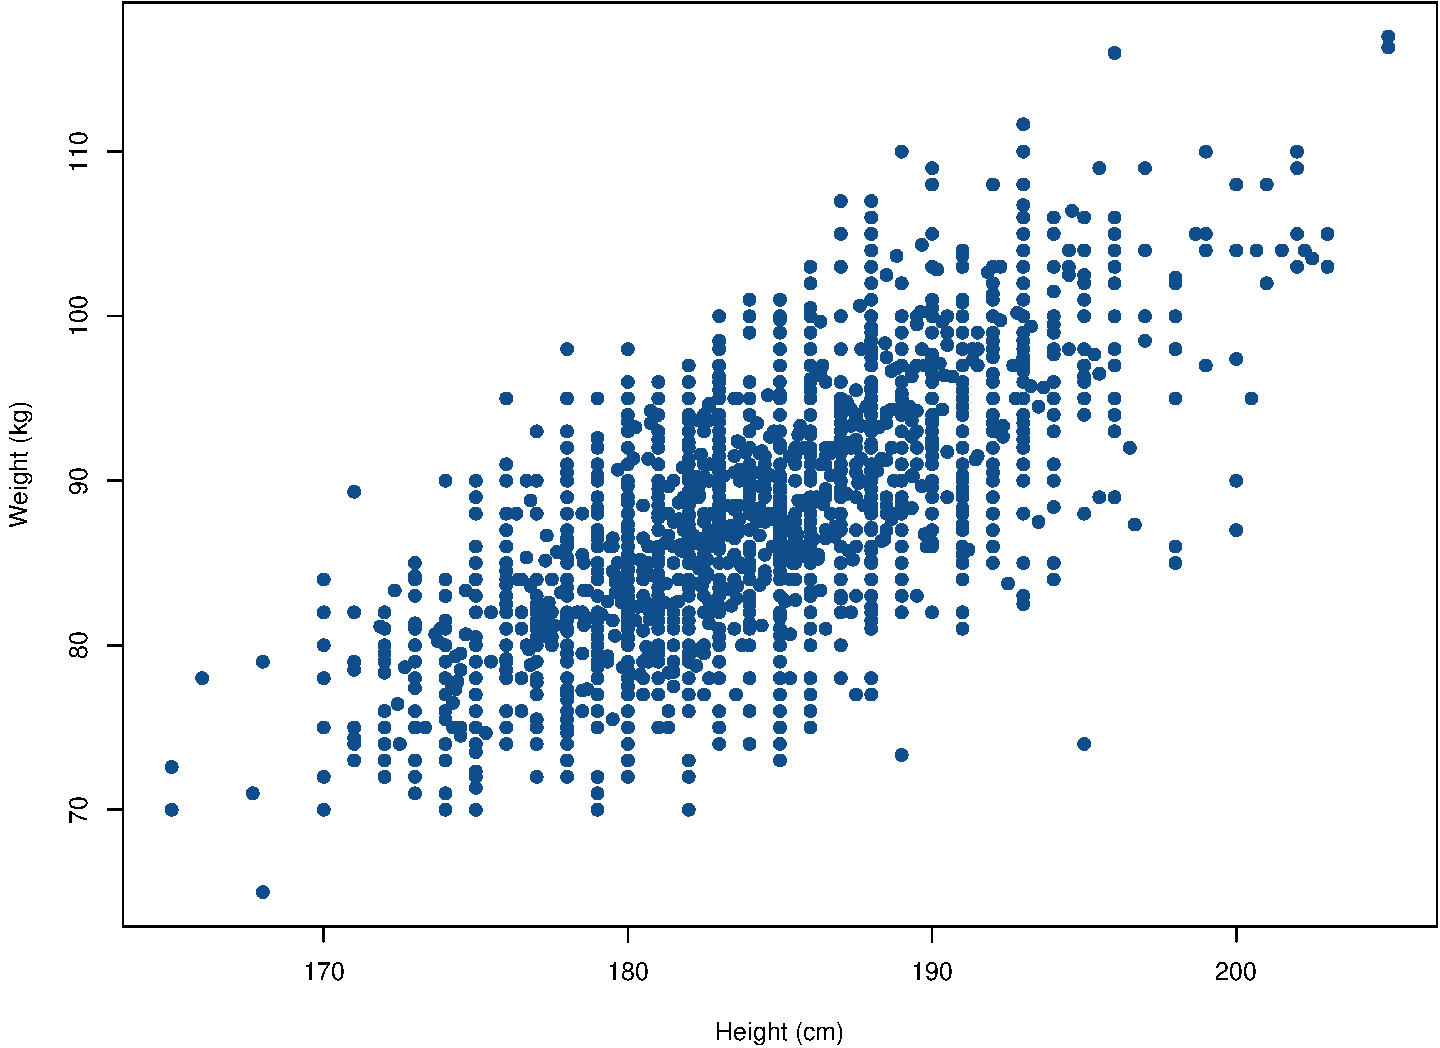
\includegraphics[height=0.85\textheight]{FIGS_slides/slides-08-hockey_players_raw}
    \end{center}
\end{frame}

\begin{frame}{Centre the data}
    \framesubtitle{Subtract the mean (our first -- simple -- change of basis)}
    \begin{center}
        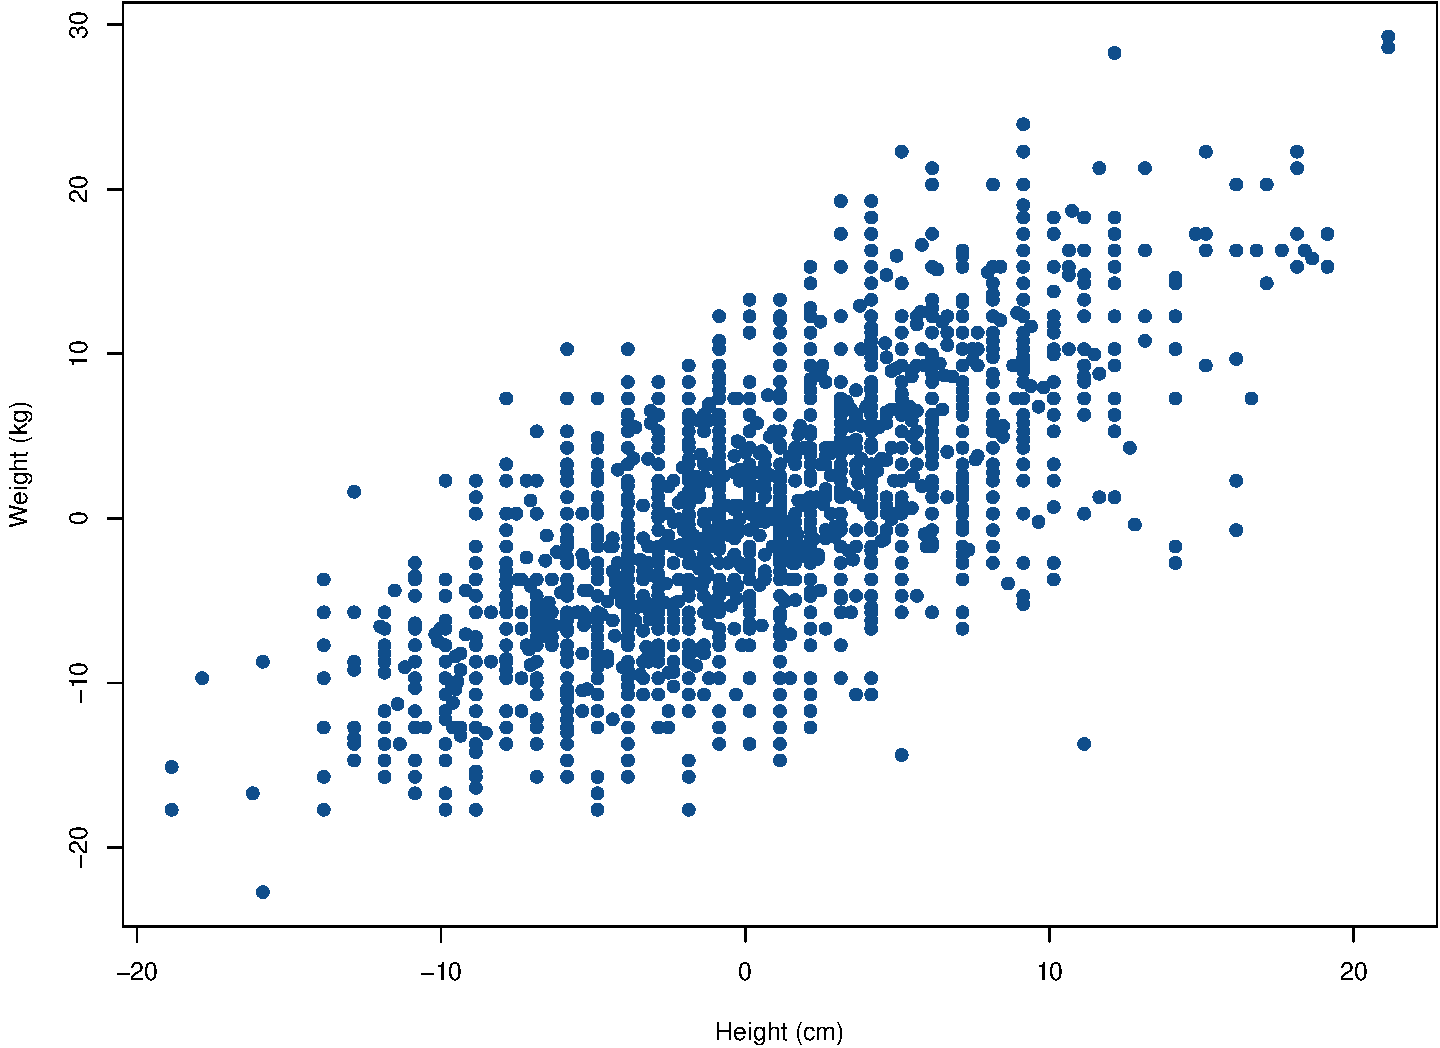
\includegraphics[height=0.85\textheight]{FIGS_slides/slides-08-hockey_players_centred}
    \end{center}
\end{frame}


\end{document}